%% survfcbf -- Application Note for Oxford Bioinformatics.
%%
%% Format: official OUP authoring template (oup-authoring-template, CTAN v1.5),
%% options [unnumsec,namedate,webpdf,contemporary,large] = the journal's two-column
%% large format with author-year citations. Limit for Application Notes: up to
%% 4 pages, approx. 2,000 words plus one figure. Structured abstract
%% (Motivation / Results / Availability and implementation). The application name
%% must appear in the title. Software public at a stable URL AT SUBMISSION and
%% archived with a DOI (Zenodo); available for two years post-publication.
%%
%% The class and the oup-abbrvnat.bst ship with TinyTeX via
%%   tlmgr install oup-authoring-template
%%
%% The text lives in pieces shared with the preprint (preprint.tex): macros.tex,
%% abstract.tex and body.tex. This file holds only what is specific to the journal
%% format. The supplementary material is supplementary.tex.
%%
%% Every number quoted in the text traces to paper/results/paper_statistics.json or to
%% a CSV tracked under experiments/benchmark/results/. Do not edit a number without
%% regenerating its source. After any edit run
%%   Rscript --no-init-file paper/check_manuscript_numbers.R
%% which checks every quoted figure against the JSON and exits non-zero on a mismatch.
\documentclass[unnumsec,namedate,webpdf,contemporary,large]{oup-authoring-template}

% URLs (GitHub, DOIs) must break inside the narrow columns, or they overflow
\usepackage{xurl}

\newcommand{\societylogo}{}

% Macros shared by appnote.tex, supplementary.tex and preprint.tex.
\newcommand{\pkg}[1]{\textsf{#1}}
\newcommand{\code}[1]{\texttt{#1}}
% Zenodo DOI of the archived software version (v0.1.0, from the GitHub release)
\newcommand{\zenododoi}{10.5281/zenodo.24472792}
% separate data record: METABRIC snapshot under ODbL-1.0 (cBioPortal licence of brca_metabric)
\newcommand{\metabricdoi}{10.5281/zenodo.24473297}
\newcommand{\pkgversion}{0.1.0}


\begin{document}

\journaltitle{Bioinformatics}
\DOI{DOI added during production}
\copyrightyear{2026}
\pubyear{2026}
\vol{XX}
\issue{x}
\access{Published: Date added during production}
\appnotes{Application Note}

\firstpage{1}

\subtitle{Gene expression}

\title[survfcbf: FCBF feature selection for survival data]{\pkg{survfcbf}:
fast correlation-based filter feature selection for right-censored survival data}

\author[1,$\ast$]{Carlos Fernandez-Lozano\ORCID{0000-0003-0413-5677}}

\address[1]{\orgdiv{Department of Computer Science and Information Technologies,
Faculty of Computer Science}, \orgname{Universidade da Coru\~na},
\orgaddress{\postcode{15071}, \state{A Coru\~na}, \country{Spain}}}

\corresp[$\ast$]{Corresponding author.
\href{mailto:carlos.fernandez@udc.es}{carlos.fernandez@udc.es}}

\received{Date}{0}{Year}
\revised{Date}{0}{Year}
\accepted{Date}{0}{Year}

\abstract{
% Abstract shared by appnote.tex and preprint.tex. Each wrapper adds its own
% Supplementary information line. Numbers are checked by
% paper/check_manuscript_numbers.R.
\textbf{Motivation:} Filter feature selection for high-dimensional survival
data is dominated by rankers, which at their conventional cut-off carry thousands
of genes forward, and adjacent ranks are often near-duplicates of one another. The
fast correlation-based filter (FCBF) addresses this in classification by
pruning each feature that an approximate Markov blanket renders redundant, returning
a compact panel. The reference benchmark of survival filters contains no method that
prunes by Markov blanket, and no FCBF implementation accepts a censored outcome.\\
\textbf{Results:} \pkg{survfcbf} carries FCBF to right-censored data through
martingale residuals of a null Cox model, with the information-theoretic core
validated against the original FCBF package (identical selections on 395
datasets). The package ships the filter in two cardinality modes,
a leakage-safe nested cross-validation harness, a survival simulator with
cluster-level ground truth, and wrappers for the standard baselines. In its
recommended mode the user sets the panel size, ten genes in our runs against roughly
two thousand for rankers at the conventional ten-percent cut-off. On eleven TCGA
cohorts and METABRIC it runs near-linearly in the number of features
($\sim p^{0.97}$, 8\,s at $p = 20{,}000$ on synthetic data) and completes every fold
on every cohort. Over ten repetitions of cross-validation, its ten-gene panels
discriminate less well than the rankers' two-thousand-gene lists, by about 0.05 in
truncated Uno's C (95\% intervals exclude zero for all three rankers, and METABRIC
shows the same gap). At equal panel size it is practically equivalent to mRMR in
discrimination and halves the within-panel redundancy of unpruned mutual information,
at a cost in selection stability.\\
\textbf{Availability and implementation:} R package, GPL-3. Source and issue
tracker at \url{https://github.com/cafernandezlo/survfcbf}, version \pkgversion{}
archived at \href{https://doi.org/\zenododoi}{doi:\zenododoi}. All benchmark result
tables regenerate from the repository.\\
\textbf{Contact:} \texttt{carlos.fernandez@udc.es}\\

% the trailing \\ gives the class's closing dot-leader its own line; without it the
% leader overflows the text block by 248pt (the only overfull the official sample
% does not also produce)
\textbf{Supplementary information:} Supplementary data are available online.\\}

\maketitle

% Main text shared by appnote.tex (journal format) and preprint.tex (preprint
% format), from the Introduction to the Conflict of interest statement. Every
% number is checked by paper/check_manuscript_numbers.R.
\section{Introduction}

The reference benchmark of filter feature selection for high-dimensional gene
expression survival data \citep{bommert2021bib} compares fourteen filters across
eleven TCGA cohorts. All fourteen are rankers, which score features marginally
or with an averaged redundancy penalty. At the conventional ten-percent cut-off
they carry more than two thousand genes forward, and because co-expressed genes
receive similar scores, the resulting lists are internally redundant.

The fast correlation-based filter \citep[FCBF;][]{yu2003, yu2004} takes a
different route. After a relevance stage based on symmetrical uncertainty (SU),
a feature $F_j$ is removed whenever some more relevant feature $F_i$ satisfies
$\mathrm{SU}(F_i, F_j) \ge \mathrm{SU}(F_j, Y)$, i.e.\ when $F_i$ approximates a
Markov blanket for $F_j$. The survivors form a compact panel, at near-linear cost,
whose size the original algorithm sets through its relevance threshold. Two decades of use in
classification have not produced a version for censored outcomes: no published
FCBF accepts a survival target, and the survival benchmark above contains no
Markov-blanket-based method at all.

\pkg{survfcbf} fills that gap, and packages with it the evaluation machinery
needed to study any survival filter without information leakage: a nested
cross-validation harness, a block-correlated simulator with known ground truth,
and uniform wrappers for the established baselines. It builds on the \pkg{mlr3}
framework \citep{lang2019} rather than duplicating it, with \pkg{mlr3proba}
supplying the survival tasks, learners and scoring the harness consumes
\citep{sonabend2021}. The ecosystem's filter collection, \pkg{mlr3filters}, does
not cover this case: its mutual-information criteria with a redundancy term (mRMR
and related filters) accept only classification and regression tasks, and none
of its filters for censored outcomes (univariate Cox and CAR scores, or the
importance of a fitted survival model) uses a Markov-blanket criterion. What
\pkg{survfcbf} adds is a filter for censored outcomes that prunes by approximate
Markov blankets, a
selector benchmark that keeps every data-dependent step inside the training
fold, and simulated ground truth at the level of correlated gene clusters.

\section{Implementation}

\paragraph{The filter.} A covariate-free Cox model \citep{therneau2000} supplies
martingale residuals as an uncensored pseudo-target, the route the reference
benchmark uses to feed mutual-information filters \citep{bommert2021bib}.
Residuals and features are discretised into equal-frequency bins ($q = 10$ by
default), and FCBF runs on the discretised data with SU throughout. Every pruning
decision is kept: each panel gene is returned with the genes it rendered redundant,
together with the two SU values behind each decision (\verb|sel$trace|). Two
cardinality modes are exposed. The original
formulation thresholds relevance at $\delta$, set by a permutation null of the
target ($B = 200$ permutations). The \code{top}-$K$ mode replaces only the
threshold: SU relevance and Markov-blanket pruning proceed unchanged until $K$
predominant features are retained. The permutation mode is faithful to the
original algorithm but under-selects when events are scarce: it returned an
empty panel in every fold for 46\% of our 300 simulated datasets and failed on
six of eleven TCGA cohorts (Supplementary Section~S7). The \code{top}-$K$ mode is
deterministic, independent of feature order (relevance ties, frequent at $q = 2$, are
broken by the absolute Spearman correlation with the residuals) and exact (7{,}143
checks against exhaustive runs). It is the mode we recommend and characterise below,
always at $q = 2$. With heavy censoring the upper residual class then also holds the
censored patients with the shortest follow-up, so relevance partly reflects
follow-up. Yet in no TCGA cohort, nor in METABRIC, does the panel predict censoring
beyond the 95th percentile of 100 random ten-gene panels, while finer binning does in
five of eleven cohorts (Supplementary Section~S2).

\paragraph{Correctness.} The information-theoretic core is validated against the
\pkg{FCBF} package \citep{fcbfbioc} on classification data, where
both should agree: SU values match to $10^{-15}$ and selections are identical on
the 395 of 400 simulated datasets without an exact SU tie and on a 19{,}541-gene
single-cell dataset at five thresholds. The single divergence arises at exact SU
ties (all 33 mismatches in a further sweep of 300 datasets that allows duplicated
features), where \pkg{survfcbf} implements the published $\ge$ rule \citep{yu2003}
and the \pkg{FCBF} code does not (Supplementary Section~S8).

\paragraph{Evaluation harness.} \code{nested\_cv\_select()} evaluates any
selector--learner pair over stratified outer folds on an
\pkg{mlr3proba} task. Everything learned from
data (the null Cox model, discretisation cut-points, $\delta$, censoring
weights, baseline hyperparameters) is fit on the training fold only. This is
the failure mode that most often invalidates survival selection benchmarks, and
the harness makes it structurally impossible. It also
flags folds in which the learner ignored its features and fell back to the null
model, which a cross-validated ridge Cox at its default one-standard-error
penalty does silently when events are scarce. Reported
metrics are Uno's C \citep{uno2011} truncated at the 80th percentile of the training
follow-up, the integrated Brier score \citep{graf1999}, correlation-aware selection
stability \citep{nogueira2018}, panel size and selection runtime, each averaged over ten
repetitions of five-fold cross-validation. Untruncated, the censoring weights of Uno's C
explode for test events beyond the training follow-up, and the value moved by more than
0.10 in 18.5\% of our folds. Cross-cohort comparison uses the Bayesian
signed-rank test with a region of practical equivalence of $\pm 0.02$ in
Uno's C and $\pm 0.05$ in stability, deciding a region when it is the largest in more
than 95\% of posterior draws \citep{benavoli2017}, reported with the power context of
\citet{boulesteix2017}: with the spread of paired C differences between cohorts (SD
$0.038$), eleven cohorts give a paired test 80\% power for differences of about $0.03$,
and the 0.95 rule reaches 79\% power only at $0.05$. Every run is reproducible from one master seed (Supplementary Section~S1).

\paragraph{Usage.} The filter is one call, and so is its evaluation:

{\small
\begin{verbatim}
library(survfcbf)
sel <- survfcbf_select(time, status, X,
                       q = 2, top = 10)
sel$selected    # column indices of the panel

library(mlr3proba); library(mlr3extralearners)
task <- surv_task(time, status, X)
bm <- benchmark_selectors(task,
    selectors = default_selectors(topk = 10)[
      c("survfcbf_topk", "variance", "carss")],
    learner   = mlr3::lrn("surv.cv_glmnet",
                alpha = 0, s = "lambda.min"),
    outer_folds = 5, seed = 1)
# Uno's C, IBS, stability, size, time
\end{verbatim}
}

\paragraph{Simulator and baselines.} \code{simulate\_dataset()} generates
block-correlated features (driver clusters with redundant members, correlated
distractors, noise), optional empirical marginals from a reference expression
matrix, event times under proportional hazards or accelerated failure time, and
censoring calibrated to a target fraction. Because redundant cluster members are
interchangeable, recovery is scored at cluster level. Wrappers cover the
variance filter, correlation-adjusted regression scores, the
mutual-information family, penalised Cox and random survival forests, so all
baselines run under the identical leakage-safe protocol. In simulation at
matched size (three or ten genes), \code{top}-$K$ recovers 0.63 and 0.78 of
the driver clusters against at most 0.34 and 0.55 for the rankers and mRMR at their
default binning, and never selects two members of one cluster. mRMR on the same two-bin
target comes close (0.61 and 0.76, with almost no copies), so the binning accounts for
most of the gain. The simulator also builds in the structure the pruning assumes, so
this shows the mechanism, not a real-data benefit (Supplementary Section~S7).

\section{Characterisation on real data}

We ran the full stack on the eleven TCGA cohorts of the reference benchmark
($p = 22{,}313$--$26{,}814$, $n = 124$--$735$, 52--152 events) and on METABRIC
\citep{metabric2012,metabric2016,metabric2019} as an independent cohort
($p = 19{,}839$, $n = 1{,}979$, 1{,}143
events), with overall survival as the endpoint throughout (Figure~\ref{fig:overview}).

\pkg{survfcbf} returns panels of 1.8 features (permutation mode) or a fixed
user budget (ten, in our runs) against 2{,}398 for the rankers at the
conventional ten-percent cut-off (1{,}984 on METABRIC) and 15.9 for penalised Cox.
On synthetic data with $n = 300$, selection cost scales as $p^{0.97}$, 8.2\,s at
twenty thousand features. In \code{top}-$K$ mode it completed every fold of every
cohort, and no ranker did better.

The honest limits. Averaged over ten five-fold splits, the three rankers at their own
cardinality discriminate better than the ten-gene \code{top}-$K$ panel, by 0.044 to
0.048 in truncated Uno's C (0.569 against 0.613 to 0.617, with 95\% intervals of the
paired differences excluding zero). The 0.95 rule decides all three comparisons at the
$\pm 0.02$ ROPE, though not at $\pm 0.03$. METABRIC shows the same gap in all ten splits
(0.044 to 0.049), and there the panel adds nothing to a clinical model of age, NPI, ER,
HER2 and PAM50 subtype (+0.003, SE 0.005). Holding panel size fixed between 5 and 20
genes (Supplementary Section~S5), \pkg{survfcbf} is 0.017 to 0.029 ahead of the
variance filter and 0.013 to 0.014 behind mutual information, neither decided, and
practically equivalent to mRMR at every size. Against mutual information on the same
two-bin target, pruning halves the within-panel redundancy (mean $|r|$ 0.134 against
0.261 at ten genes, lower in all eleven cohorts), a level that mRMR (0.121) and
correlation-adjusted scores (0.105) also reach. The pruning costs stability:
\pkg{survfcbf} (0.105 at ten genes) is less stable than mutual information on the same
target (0.141), matches mRMR on it (0.108), beats mRMR at its default binning (0.021) and
stays far below correlation-adjusted scores (0.279), and this ordering holds at every
similarity threshold from 0.5 to 0.9. A ten-gene panel buys size and
cost, not pathway coverage, and it is not a validated prognostic signature. Users who
need a stable ranking, or the best discrimination whatever the panel size, should use
the ranker baselines the package wraps. \pkg{survfcbf} is for the regime where a
compact panel, pruned by approximate Markov blankets and cheaply obtained, is the
object of interest.

\begin{figure*}[t]
\centering
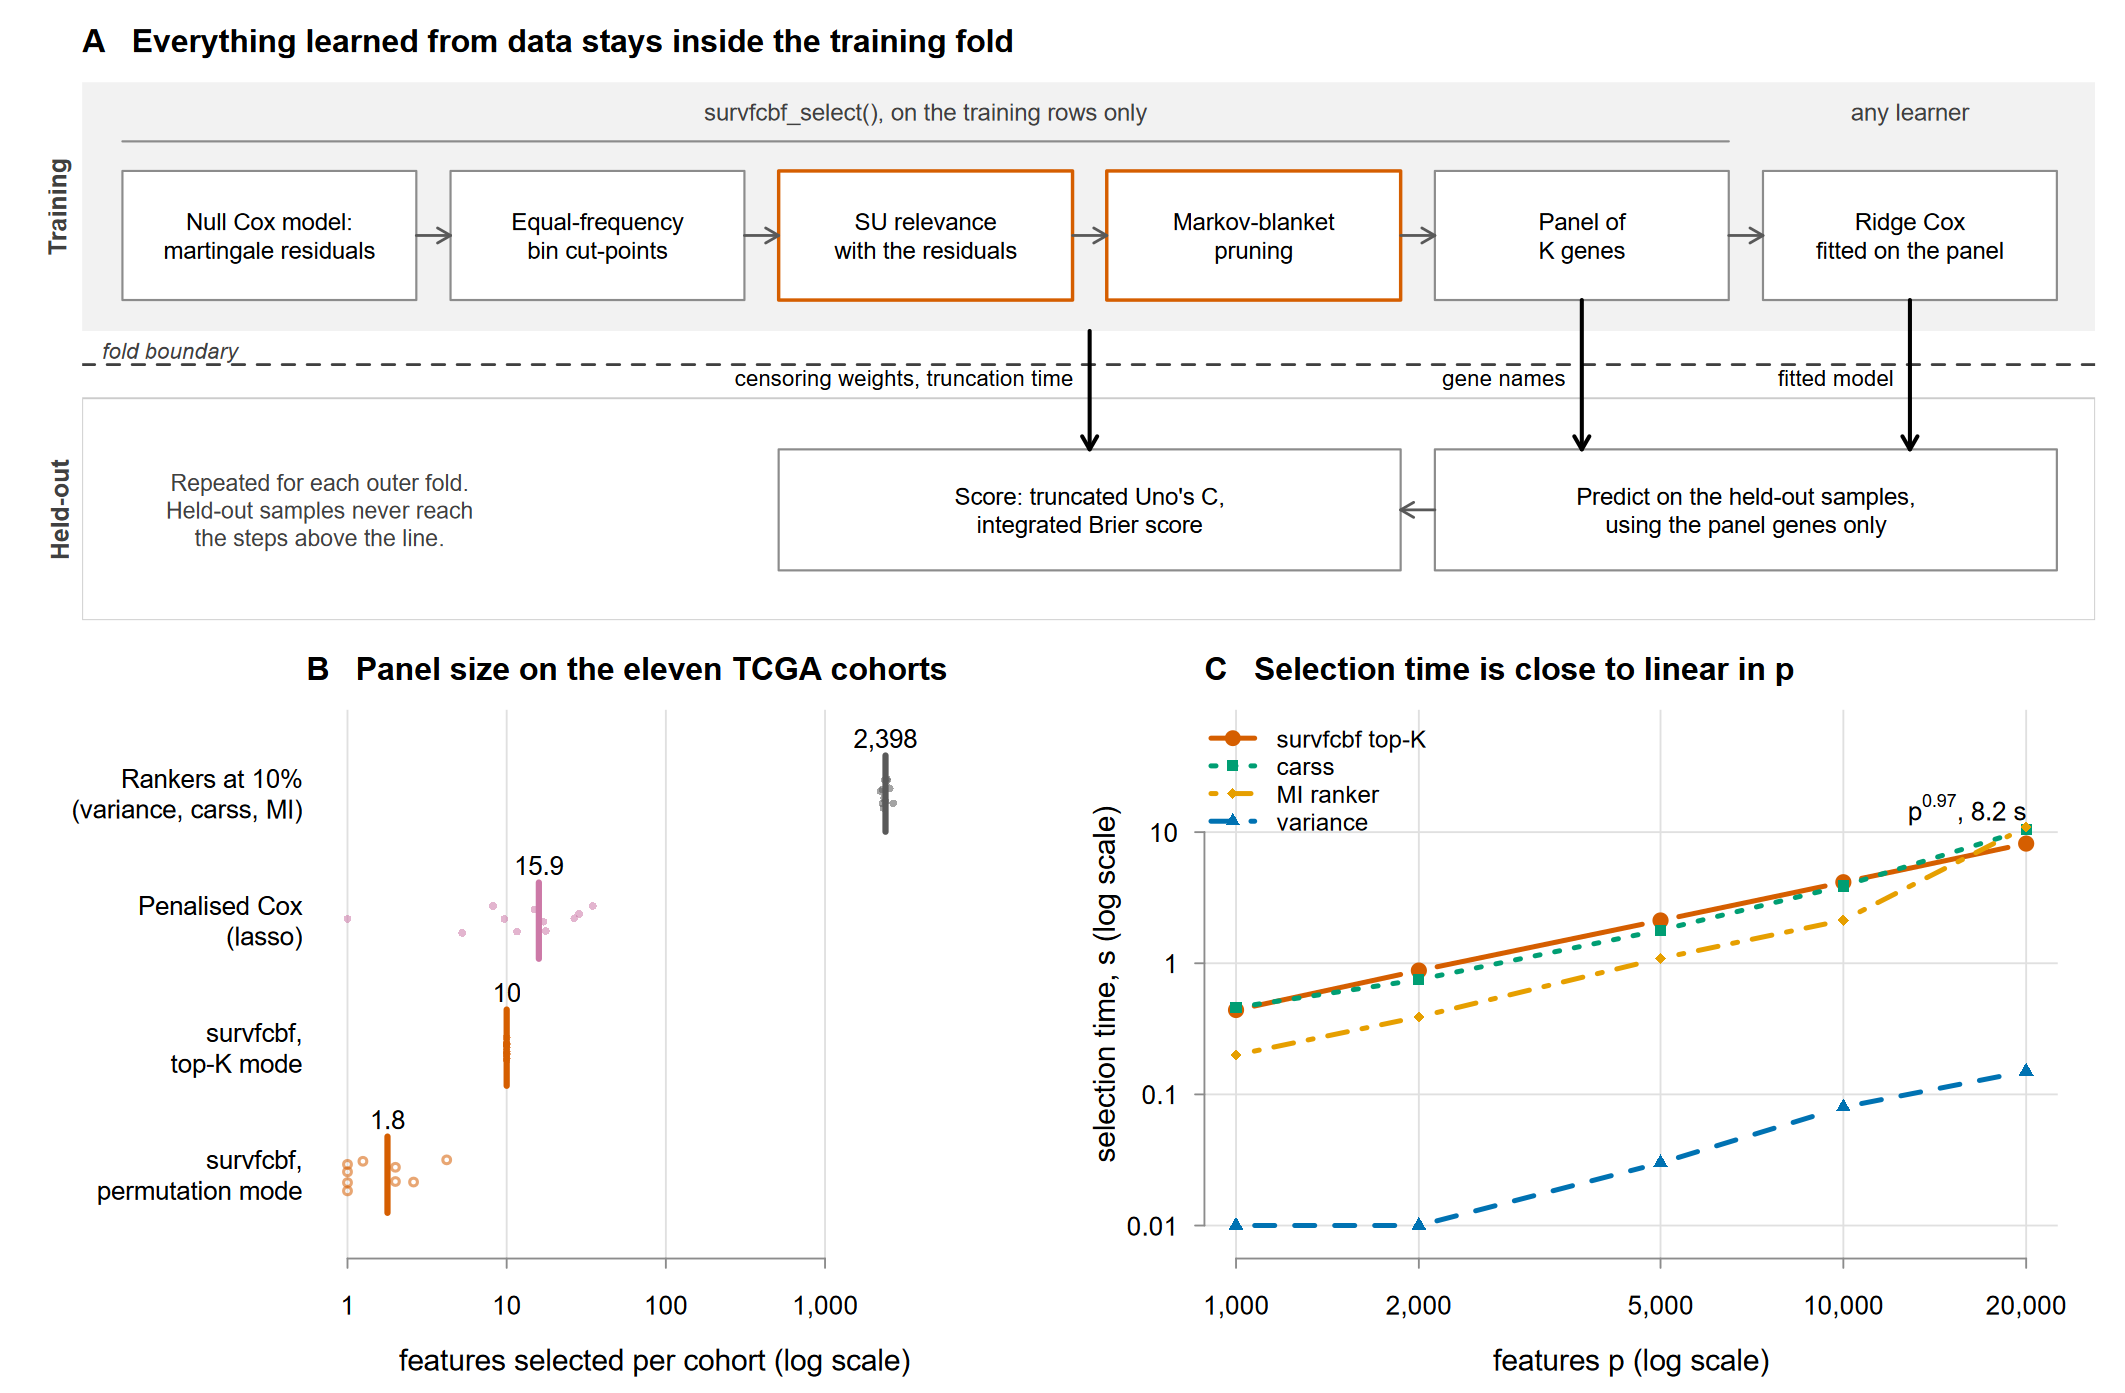
\includegraphics[width=\textwidth]{Figure_appnote.png}
\caption{\textbf{\pkg{survfcbf} and its evaluation harness.}
(\textbf{A})~What crosses the fold boundary in nested cross-validation: only the
gene names, the fitted model, the censoring weights and the truncation time reach the
held-out samples.
The two stages specific to FCBF are outlined in orange.
(\textbf{B})~Panel size at the conventional cut-offs on the eleven TCGA cohorts
(dots) and their mean (ticks), except two cohorts with no permutation-mode panel.
(\textbf{C})~Selection time on synthetic data, $n = 300$.}
\label{fig:overview}
\end{figure*}

\section{Conclusion}

\pkg{survfcbf} makes the approximate-Markov-blanket family available for
censored outcomes for the first time, inside an evaluation stack that treats
leakage, seeding and honest cross-cohort inference as package responsibilities,
so that a new filter enters the same protocol through one function call, and every
number reported here is recomputed from result files tracked in the repository.

\section{Availability and implementation}

\pkg{survfcbf} is an R package under GPL-3. Development and issues:
\url{https://github.com/cafernandezlo/survfcbf}. The submitted version
(\pkgversion) and its result tables are archived at
\href{https://doi.org/\zenododoi}{doi:\zenododoi}. The eleven TCGA cohorts are
the OpenML datasets prepared by \citet{herrmann2020} and selected for the
reference benchmark \citep{bommert2021bib}, with their identifiers listed in the
repository. METABRIC expression is the complete cBioPortal
\citep{cerami2012,gao2013,debruijn2023} profile \code{brca\_metabric\_mrna} of
study \code{brca\_metabric} (19{,}850 genes, 1{,}980 samples), retrieved through
the cBioPortal REST API (portal v7.2.0) on 25 October 2026. That snapshot and the
matching clinical table are archived separately under the ODC Open Database
License v1.0, the licence of the study in cBioPortal, at
\href{https://doi.org/\metabricdoi}{doi:\metabricdoi}.

\section{Acknowledgements}

The results shown here are in whole or part based upon data generated by the
TCGA Research Network: \url{https://www.cancer.gov/tcga}. This research project
was made possible through the access granted by the Galician Supercomputing
Center (CESGA) to its supercomputing infrastructure.

\section{Funding}

Grant PID2024-162441OA-I00 funded by
MICIU/AEI/\allowbreak10.13039/\allowbreak501100011033 and by
``ERDF/EU''. RePo-SUDOE, with project reference S1/1.1/P0033, a project
co-financed by the Interreg Sudoe Programme through the European Regional
Development Fund (ERDF). Funding for open access charge: Universidade da
Coru\~na/CISUG.

\section{Conflict of interest}

None declared.


\bibliographystyle{oup-abbrvnat}
\bibliography{appnote}

\end{document}
